%  LaTeX support: latex@mdpi.com 
%  For support, please attach all files needed for compiling as well as the log file, and specify your operating system, LaTeX version, and LaTeX editor.

%=================================================================
\documentclass[diagnostics,article,submit,pdftex,moreauthors]{Definitions/mdpi} 
\usepackage{graphicx}
\usepackage{url}
\urldef{\mailsa}\path|{loz2,rrz}@aber.ac.uk|    
\newcommand{\keywords}[1]{\par\addvspace\baselineskip
\noindent\keywordname\enspace\ignorespaces#1}
\usepackage{tikz}
\usetikzlibrary{shapes.geometric, arrows}
\tikzstyle{arrow} = [thick,->,>=stealth]
\usepackage{pgfplots}
\usepackage{subfig}
\usepackage{float}
\pgfplotsset{width=8cm,compat=1.8}
\usepackage{adjustbox}
% We will externalize the figures
\usepgfplotslibrary{external}
\tikzexternalize

%--------------------
% Class Options:
%--------------------
%----------
% journal
%----------
% Choose between the following MDPI journals:
% acoustics, actuators, addictions, admsci, adolescents, aerobiology, aerospace, agriculture, agriengineering, agrochemicals, agronomy, ai, air, algorithms, allergies, alloys, analytica, analytics, anatomia, animals, antibiotics, antibodies, antioxidants, applbiosci, appliedchem, appliedmath, applmech, applmicrobiol, applnano, applsci, aquacj, architecture, arm, arthropoda, arts, asc, asi, astronomy, atmosphere, atoms, audiolres, automation, axioms, bacteria, batteries, bdcc, behavsci, beverages, biochem, bioengineering, biologics, biology, biomass, biomechanics, biomed, biomedicines, biomedinformatics, biomimetics, biomolecules, biophysica, biosensors, biotech, birds, bloods, blsf, brainsci, breath, buildings, businesses, cancers, carbon, cardiogenetics, catalysts, cells, ceramics, challenges, chemengineering, chemistry, chemosensors, chemproc, children, chips, cimb, civileng, cleantechnol, climate, clinpract, clockssleep, cmd, coasts, coatings, colloids, colorants, commodities, compounds, computation, computers, condensedmatter, conservation, constrmater, cosmetics, covid, crops, cryptography, crystals, csmf, ctn, curroncol, cyber, dairy, data, ddc, dentistry, dermato, dermatopathology, designs, devices, diabetology, diagnostics, dietetics, digital, disabilities, diseases, diversity, dna, drones, dynamics, earth, ebj, ecologies, econometrics, economies, education, ejihpe, electricity, electrochem, electronicmat, electronics, encyclopedia, endocrines, energies, eng, engproc, entomology, entropy, environments, environsciproc, epidemiologia, epigenomes, est, fermentation, fibers, fintech, fire, fishes, fluids, foods, forecasting, forensicsci, forests, foundations, fractalfract, fuels, future, futureinternet, futurepharmacol, futurephys, futuretransp, galaxies, games, gases, gastroent, gastrointestdisord, gels, genealogy, genes, geographies, geohazards, geomatics, geosciences, geotechnics, geriatrics, grasses, gucdd, hazardousmatters, healthcare, hearts, hemato, hematolrep, heritage, higheredu, highthroughput, histories, horticulturae, hospitals, humanities, humans, hydrobiology, hydrogen, hydrology, hygiene, idr, ijerph, ijfs, ijgi, ijms, ijns, ijpb, ijtm, ijtpp, ime, immuno, informatics, information, infrastructures, inorganics, insects, instruments, inventions, iot, j, jal, jcdd, jcm, jcp, jcs, jcto, jdb, jeta, jfb, jfmk, jimaging, jintelligence, jlpea, jmmp, jmp, jmse, jne, jnt, jof, joitmc, jor, journalmedia, jox, jpm, jrfm, jsan, jtaer, jvd, jzbg, kidneydial, kinasesphosphatases, knowledge, land, languages, laws, life, liquids, literature, livers, logics, logistics, lubricants, lymphatics, machines, macromol, magnetism, magnetochemistry, make, marinedrugs, materials, materproc, mathematics, mca, measurements, medicina, medicines, medsci, membranes, merits, metabolites, metals, meteorology, methane, metrology, micro, microarrays, microbiolres, micromachines, microorganisms, microplastics, minerals, mining, modelling, molbank, molecules, mps, msf, mti, muscles, nanoenergyadv, nanomanufacturing,\gdef\@continuouspages{yes}} nanomaterials, ncrna, ndt, network, neuroglia, neurolint, neurosci, nitrogen, notspecified, %%nri, nursrep, nutraceuticals, nutrients, obesities, oceans, ohbm, onco, %oncopathology, optics, oral, organics, organoids, osteology, oxygen, parasites, parasitologia, particles, pathogens, pathophysiology, pediatrrep, pharmaceuticals, pharmaceutics, pharmacoepidemiology,\gdef\@ISSN{2813-0618}\gdef\@continuous pharmacy, philosophies, photochem, photonics, phycology, physchem, physics, physiologia, plants, plasma, platforms, pollutants, polymers, polysaccharides, poultry, powders, preprints, proceedings, processes, prosthesis, proteomes, psf, psych, psychiatryint, psychoactives, publications, quantumrep, quaternary, qubs, radiation, reactions, receptors, recycling, regeneration, religions, remotesensing, reports, reprodmed, resources, rheumato, risks, robotics, ruminants, safety, sci, scipharm, sclerosis, seeds, sensors, separations, sexes, signals, sinusitis, skins, smartcities, sna, societies, socsci, software, soilsystems, solar, solids, spectroscj, sports, standards, stats, std, stresses, surfaces, surgeries, suschem, sustainability, symmetry, synbio, systems, targets, taxonomy, technologies, telecom, test, textiles, thalassrep, thermo, tomography, tourismhosp, toxics, toxins, transplantology, transportation, traumacare, traumas, tropicalmed, universe, urbansci, uro, vaccines, vehicles, venereology, vetsci, vibration, virtualworlds, viruses, vision, waste, water, wem, wevj, wind, women, world, youth, zoonoticdis 
% For posting an early version of this manuscript as a preprint, you may use "preprints" as the journal. Changing "submit" to "accept" before posting will remove line numbers.

%---------
% article
%---------
% The default type of manuscript is "article", but can be replaced by: 
% abstract, addendum, article, book, bookreview, briefreport, casereport, comment, commentary, communication, conferenceproceedings, correction, conferencereport, entry, expressionofconcern, extendedabstract, datadescriptor, editorial, essay, erratum, hypothesis, interestingimage, obituary, opinion, projectreport, reply, retraction, review, perspective, protocol, shortnote, studyprotocol, systematicreview, supfile, technicalnote, viewpoint, guidelines, registeredreport, tutorial
% supfile = supplementary materials

%----------
% submit
%----------
% The class option "submit" will be changed to "accept" by the Editorial Office when the paper is accepted. This will only make changes to the frontpage (e.g., the logo of the journal will get visible), the headings, and the copyright information. Also, line numbering will be removed. Journal info and pagination for accepted papers will also be assigned by the Editorial Office.

%------------------
% moreauthors
%------------------
% If there is only one author the class option oneauthor should be used. Otherwise use the class option moreauthors.

%---------
% pdftex
%---------
% The option pdftex is for use with pdfLaTeX. Remove "pdftex" for (1) compiling with LaTeX & dvi2pdf (if eps figures are used) or for (2) compiling with XeLaTeX.

%=================================================================
% MDPI internal commands - do not modify
\firstpage{1} 
\makeatletter 
\setcounter{page}{\@firstpage} 
\makeatother
\pubvolume{1}
\issuenum{1}
\articlenumber{0}
\pubyear{2024}
\copyrightyear{2024}
%\externaleditor{Academic Editor: Firstname Lastname}
\datereceived{ } 
\daterevised{ } % Comment out if no revised date
\dateaccepted{ } 
\datepublished{ } 
%\datecorrected{} % For corrected papers: "Corrected: XXX" date in the original paper.
%\dateretracted{} % For corrected papers: "Retracted: XXX" date in the original paper.
\hreflink{https://doi.org/} % If needed use \linebreak
%\doinum{}
%\pdfoutput=1 % Uncommented for upload to arXiv.org
%\CorrStatement{yes}  % For updates


%=================================================================
% Add packages and commands here. The following packages are loaded in our class file: fontenc, inputenc, calc, indentfirst, fancyhdr, graphicx, epstopdf, lastpage, ifthen, float, amsmath, amssymb, lineno, setspace, enumitem, mathpazo, booktabs, titlesec, etoolbox, tabto, xcolor, colortbl, soul, multirow, microtype, tikz, totcount, changepage, attrib, upgreek, array, tabularx, pbox, ragged2e, tocloft, marginnote, marginfix, enotez, amsthm, natbib, hyperref, cleveref, scrextend, url, geometry, newfloat, caption, draftwatermark, seqsplit
% cleveref: load \crefname definitions after \begin{document}

%=================================================================
% Please use the following mathematics environments: Theorem, Lemma, Corollary, Proposition, Characterization, Property, Problem, Example, ExamplesandDefinitions, Hypothesis, Remark, Definition, Notation, Assumption
%% For proofs, please use the proof environment (the amsthm package is loaded by the MDPI class).

%=================================================================
% Add packages and commands here. The following packages are loaded in our class file: fontenc, inputenc, calc, indentfirst, fancyhdr, graphicx, epstopdf, lastpage, ifthen, float, amsmath, amssymb, lineno, setspace, enumitem, mathpazo, booktabs, titlesec, etoolbox, tabto, xcolor, colortbl, soul, multirow, microtype, tikz, totcount, changepage, attrib, upgreek, array, tabularx, pbox, ragged2e, tocloft, marginnote, marginfix, enotez, amsthm, natbib, hyperref, cleveref, scrextend, url, geometry, newfloat, caption, draftwatermark, seqsplit
% cleveref: load \crefname definitions after \begin{document}

%=================================================================
% Please use the following mathematics environments: Theorem, Lemma, Corollary, Proposition, Characterization, Property, Problem, Example, ExamplesandDefinitions, Hypothesis, Remark, Definition, Notation, Assumption
%% For proofs, please use the proof environment (the amsthm package is loaded by the MDPI class).

%=================================================================
% Full title of the paper (Capitalized)
\Title{Acute Lymphocytic Leukemia Detection Using Deep Learning Methods}

% MDPI internal command: Title for citation in the left column
\TitleCitation{Acute Lymphocytic Leukemia Detection Using Deep Learning Methods}

% Author Orchid ID: enter ID or remove command
\newcommand{\orcidauthorA}{0000-0000-0000-000X} % Add \orcidA{} behind the author's name
%\newcommand{\orcidauthorB}{0000-0000-0000-000X} % Add \orcidB{} behind the author's name

% Authors, for the paper (add full first names)
\Author{Louai Zaiter $^{1,}$* and Reyer Zwiggelaar $^{1}}

%\longauthorlist{yes}

% MDPI internal command: Authors, for metadata in PDF
\AuthorNames{Louai Zaiter and Reyer Zwiggelaar}

% MDPI internal command: Authors, for citation in the left column
\AuthorCitation{Zaiter, L.; Zwiggelaar, R.;}
% If this is a Chicago style journal: Lastname, Firstname, Firstname Lastname, and Firstname Lastname.

% Affiliations / Addresses (Add [1] after \address if there is only one affiliation.)
\address[1]{%
$^{1}$ \quad Department of Computer Science, Aberystwyth University, Ceredigion, SY23 3DB}

% Contact information of the corresponding author
\corres{Correspondence: loz2@aber.ac.uk; rrz@aber.ac.uk}

% Current address and/or shared authorship
  % Current address should not be the same as any items in the Affiliation section.
% The commands \thirdnote{} till \eighthnote{} are available for further notes

%\simplesumm{} % Simple summary

%\conference{} % An extended version of a conference paper

% Abstract (Do not insert blank lines, i.e. \\) 
\abstract{ 
    This study introduces a novel computer-aided detection system to classify white blood cells as either leukocyte or healthy in microscopic images. We use binary thresholding to segment white blood cells in microscopic images. We apply the mask to each image and feed the results into convolutional neural networks. During this study, we used two publicly available datasets i.e. ALL-IDB 1 and ALL-IDB 2. The proposed lightweight convolutional neural network outperformed pre-trained models, such as ResNet50, while scoring 99\% accuracy on the first dataset and 98\% accuracy on the second dataset using a 5-fold cross validation technique.}

% Keywords
\keyword{Acute Lymphocytic Leukemia; Convolutional Neural Networks; Deep Learning; Computer-aided Detection}

% The fields PACS, MSC, and JEL may be left empty or commented out if not applicable
%\PACS{J0101}
%\MSC{}
%\JEL{}

%%%%%%%%%%%%%%%%%%%%%%%%%%%%%%%%%%%%%%%%%%
% Only for the journal Diversity
%\LSID{\url{http://}}

%%%%%%%%%%%%%%%%%%%%%%%%%%%%%%%%%%%%%%%%%%
% Only for the journal Applied Sciences
%\featuredapplication{Authors are encouraged to provide a concise description of the specific application or a potential application of the work. This section is not mandatory.}
%%%%%%%%%%%%%%%%%%%%%%%%%%%%%%%%%%%%%%%%%%

%%%%%%%%%%%%%%%%%%%%%%%%%%%%%%%%%%%%%%%%%%
% Only for the journal Data
%\dataset{DOI number or link to the deposited data set if the data set is published separately. If the data set shall be published as a supplement to this paper, this field will be filled by the journal editors. In this case, please submit the data set as a supplement.}
%\datasetlicense{License under which the data set is made available (CC0, CC-BY, CC-BY-SA, CC-BY-NC, etc.)}

%%%%%%%%%%%%%%%%%%%%%%%%%%%%%%%%%%%%%%%%%%
% Only for the journal Toxins
%\keycontribution{The breakthroughs or highlights of the manuscript. Authors can write one or two sentences to describe the most important part of the paper.}

%%%%%%%%%%%%%%%%%%%%%%%%%%%%%%%%%%%%%%%%%%
% Only for the journal Encyclopedia
%\encyclopediadef{For entry manuscripts only: please provide a brief overview of the entry title instead of an abstract.}

%%%%%%%%%%%%%%%%%%%%%%%%%%%%%%%%%%%%%%%%%%
% Only for the journal Advances in Respiratory Medicine
%\addhighlights{yes}
%\renewcommand{\addhighlights}{%

%\noindent This is an obligatory section in “Advances in Respiratory Medicine”, whose goal is to increase the discoverability and readability of the article via search engines and other scholars. Highlights should not be a copy of the abstract, but a simple text allowing the reader to quickly and simplified find out what the article is about and what can be cited from it. Each of these parts should be devoted up to 2~bullet points.\vspace{3pt}\\
%\textbf{What are the main findings?}
% \begin{itemize}[labelsep=2.5mm,topsep=-3pt]
% \item First bullet.
% \item Second bullet.
% \end{itemize}\vspace{3pt}
%\textbf{What is the implication of the main finding?}
% \begin{itemize}[labelsep=2.5mm,topsep=-3pt]
% \item First bullet.
% \item Second bullet.
% \end{itemize}
%}

%%%%%%%%%%%%%%%%%%%%%%%%%%%%%%%%%%%%%%%%%%
\begin{document}

%%%%%%%%%%%%%%%%%%%%%%%%%%%%%%%%%%%%%%%%%% %% Remove this when starting to work on the template.

\section{Introduction}
According to \cite{key}, Acute Lymphocytic Leukemia (ALL) is a type of cancer in which the bone marrow makes a lot of white blood cells specifically lymphocytes. These cells cannot work normally and are known as blast cells. 

This study introduces a novel machine-learning algorithm to segment and classify microscopic blood images. The proposed method is composed of four steps; (1) Thresholding \cite{kohler1981segmentation}, (2) Region of interest extraction, (3) feature extraction, and (4) classification. The novelty of our work consists of the proposed lightweight convolutional neural network \cite{o2015introduction} (CNN) model that is used to extract deep features using a small number of input images. The features are classified using a fully connected network (FCN) that consists of a dense layer, an exponential linear unit \cite{clevert2015fast} (ELU) layer, and a softmax layer with two neurons. We compared the results of our proposed method with those of pre-trained CNNs and we found that the lightweight CNN outperforms all other models while scoring better accuracy, precision, and recall in a significantly short amount of time. 

%The rest of the paper is organized as follows; Section 2 presents some of the related works. Section 3 is about the dataset. Section 4 introduces the methodology and the novel machine-learning algorithm. The results and findings are presented in Section 5. The last section is a conclusion.

\section{Related Work}
Khandekar et al. \cite{khandekar2021automated} introduced an object detection model that uses a YOLOv4 architecture to detect and classify blast cells. Their proposed method achieved 96.06\% on the All-IDB1 dataset and 98.7\% on the C\_NMC\_2019 dataset. Ahmed et al. \cite{ahmed2019identification} introduced a deep learning algorithm to classify microscopic blood images taken from ALL-IDB1 and ASH datasets. They compared the performance of their proposed CNN with those of traditional machine learning methods such as decision trees, k-nearest neighbors \cite{peterson2009k}, and support vector machines \cite{hearst1998support}. To evaluate their method, they used 5-fold cross-validation. Their proposed model achieved 88.25\% in detecting leukemia and 81.71\% in multi-class classification of all subtypes. Arif et al. \cite{arif2022automatic} introduced a deep-learning pipeline to classify images from the ALL-IDB dataset. As a classifier and feature extractor they fine-tuned an AlexNet \cite{krizhevsky2012imagenet} model. To segment blood microscopic images, they used a network with three convolutional layers. Each one is succeeded by batch normalization, Leaky ReLU, and max-pooling layer. Their proposed algorithm reached 98\% of accuracy. Sulaiman et al. \cite{sulaiman2023resrandsvm} introduced a hybrid machine learning algorithm to classify lymphocytes into leukocytes or normal. Their pipeline consists of the following steps; features extraction, feature selection, and classification. To extract deep learned feature, they tried several pretrained models and found that the ResNet50 has given the best performance. As feature selector, they used a random forest classifier to evaluate the imporant of each feature then they selected the best 584 features out of 2048 features. As a classifier, the support vector machine has resulted in the best performance i.e 90\% of accuracy. Mohammed et al. \cite{mohammed2013chronic} presented a novel segmentation algorithm to extract cells and nuclei from microscopic blood images. Their proposed method used Otsu thresholding, canny edge detection, and watershed segmentation methods. Lu et al. \cite{lu2021wbc} proposed a white blood cells segmentation algorithm that consists of a combination of UNet++ and ResNet. Their proposed netwrok outperformed all state-of-the-art models and reached a dice coefficient of 99.28\%. 
\section{Dataset}
We use two publicly available datasets i.e. ALL-IDB 1 and ALL-IDB 2 \cite{labati2011all}.\\
The first dataset contains microscopic blood images of 108 patients. 39 images are from patients having acute lymphocytic leukemia and 59 samples are from healthy patients. All lymphocytes have been labeled by expert oncologists. The number of candidate lymphoblasts present in the dataset is 510.\\
The second dataset includes microscopic images of single lymphocytes. The dataset contains 260 images that are divided into two classes i.e 130 microscopic images of patient suffering from leukemia and 130 images of normal cases. 


\section{Methodology}
\begin{figure}[htp]
  \centering
  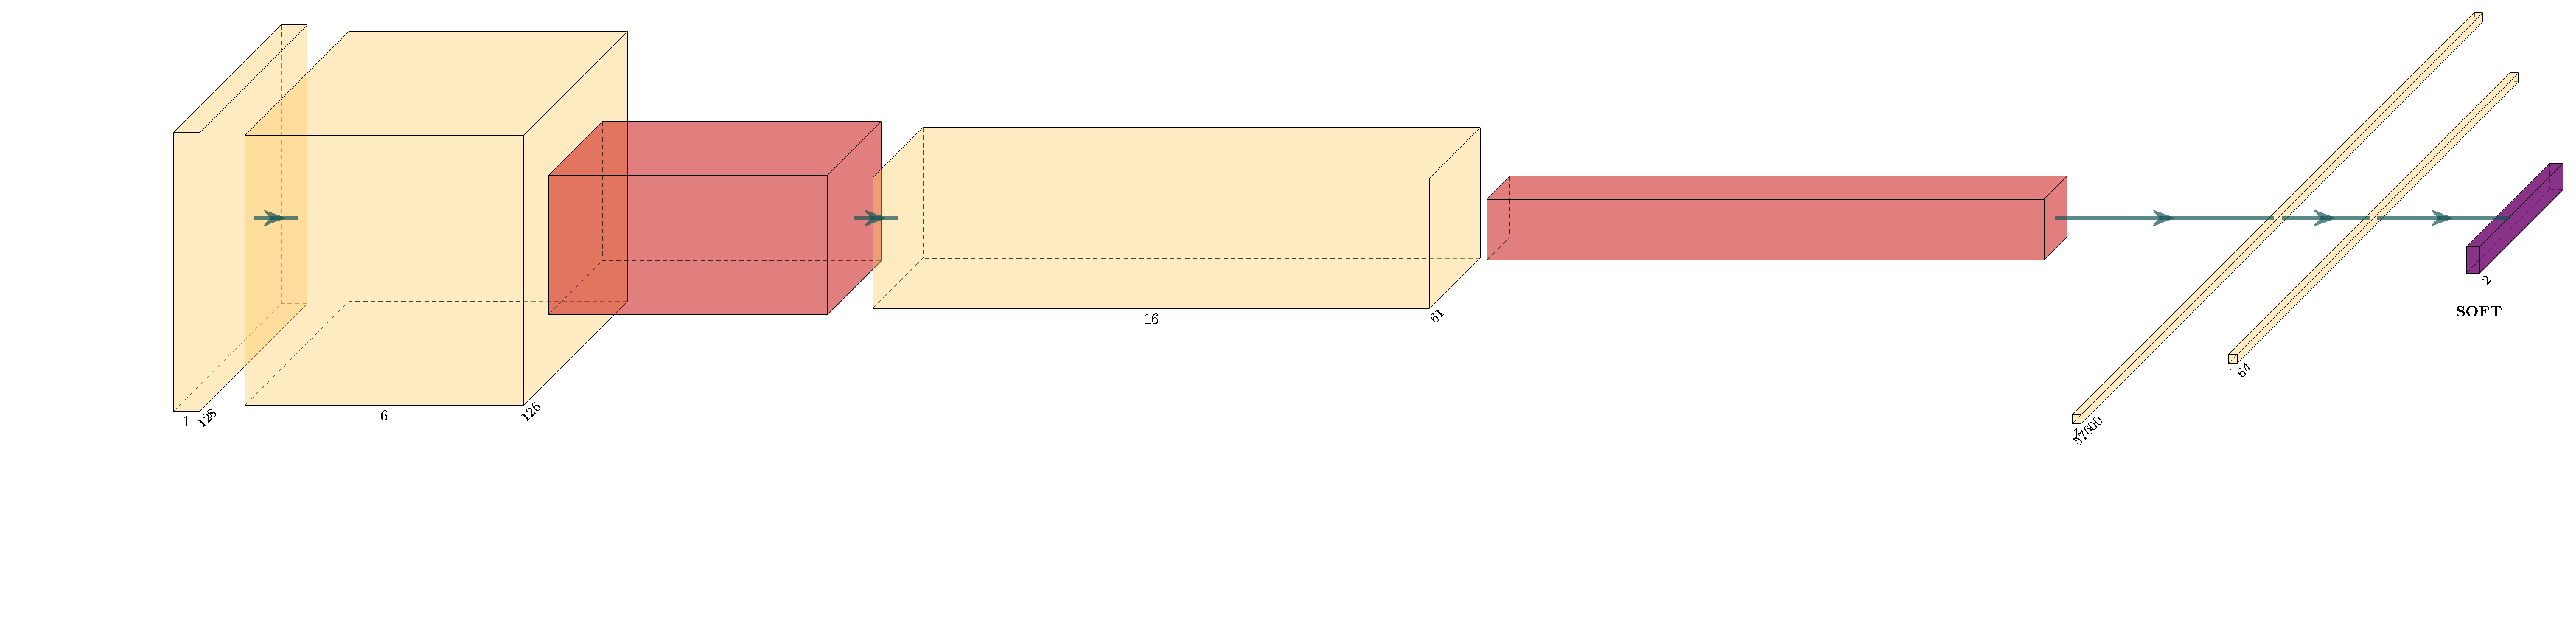
\includegraphics[width=10cm]{images/graph.pdf}
  \caption{The proposed Lightweight CNN architecture that consists of two convolutional layers each one is succeeded by a max pooling layer. The last part is a fully connected network with a softmax activation function and two output neurons.}
\end{figure}
\subsection{Thresholding}
During this study, we consider using binary thresholding to separate the white blood cells from other cells available in the microscopic image. If we draw the histogram to analyze the frequency of each pixel color within grayscale images, we find that there are three peaks; the first one is for white blood cells. The second one is for red blood cells and the third one is for the background. A good approach to threshold the images is to cluster the pixels into three sets, then, select the highest value from the cluster having the least frequency which corresponds to the white blood cells cluster.

\begin{figure}[!h]
  \centering
  \subfloat[]{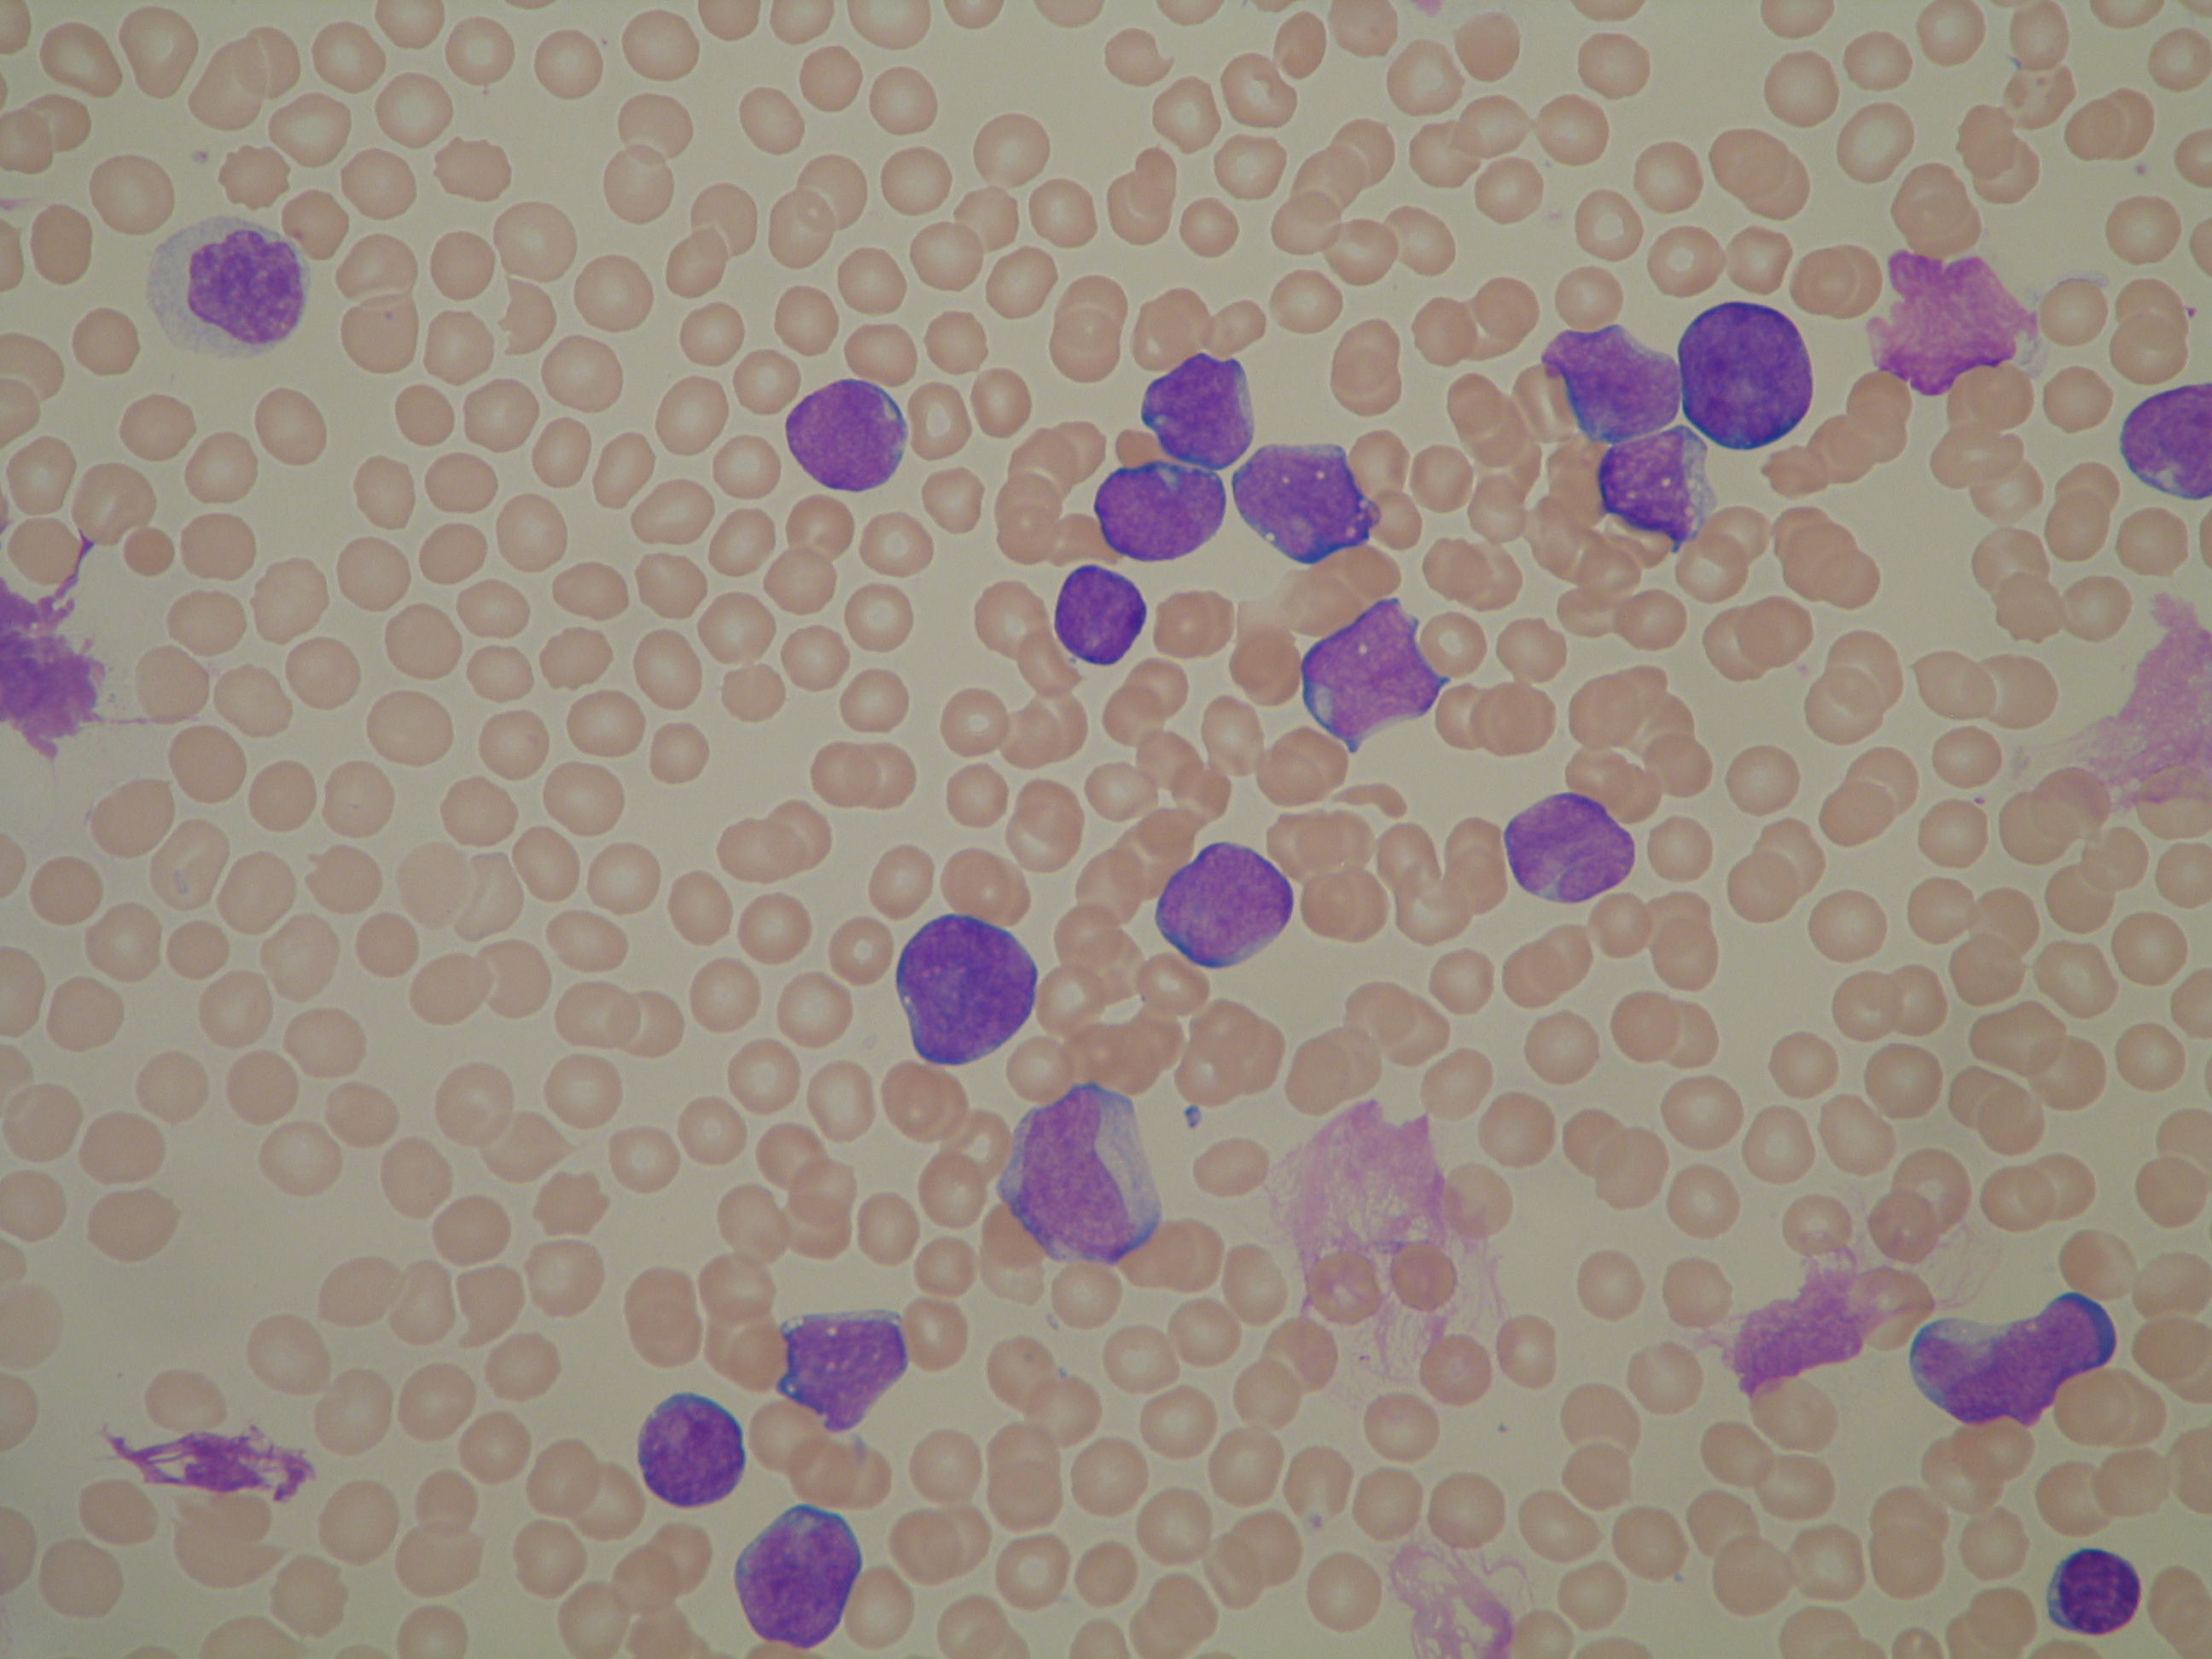
\includegraphics[width=3cm]{images/Im048_1.jpg}}
  \quad 
  \subfloat[]{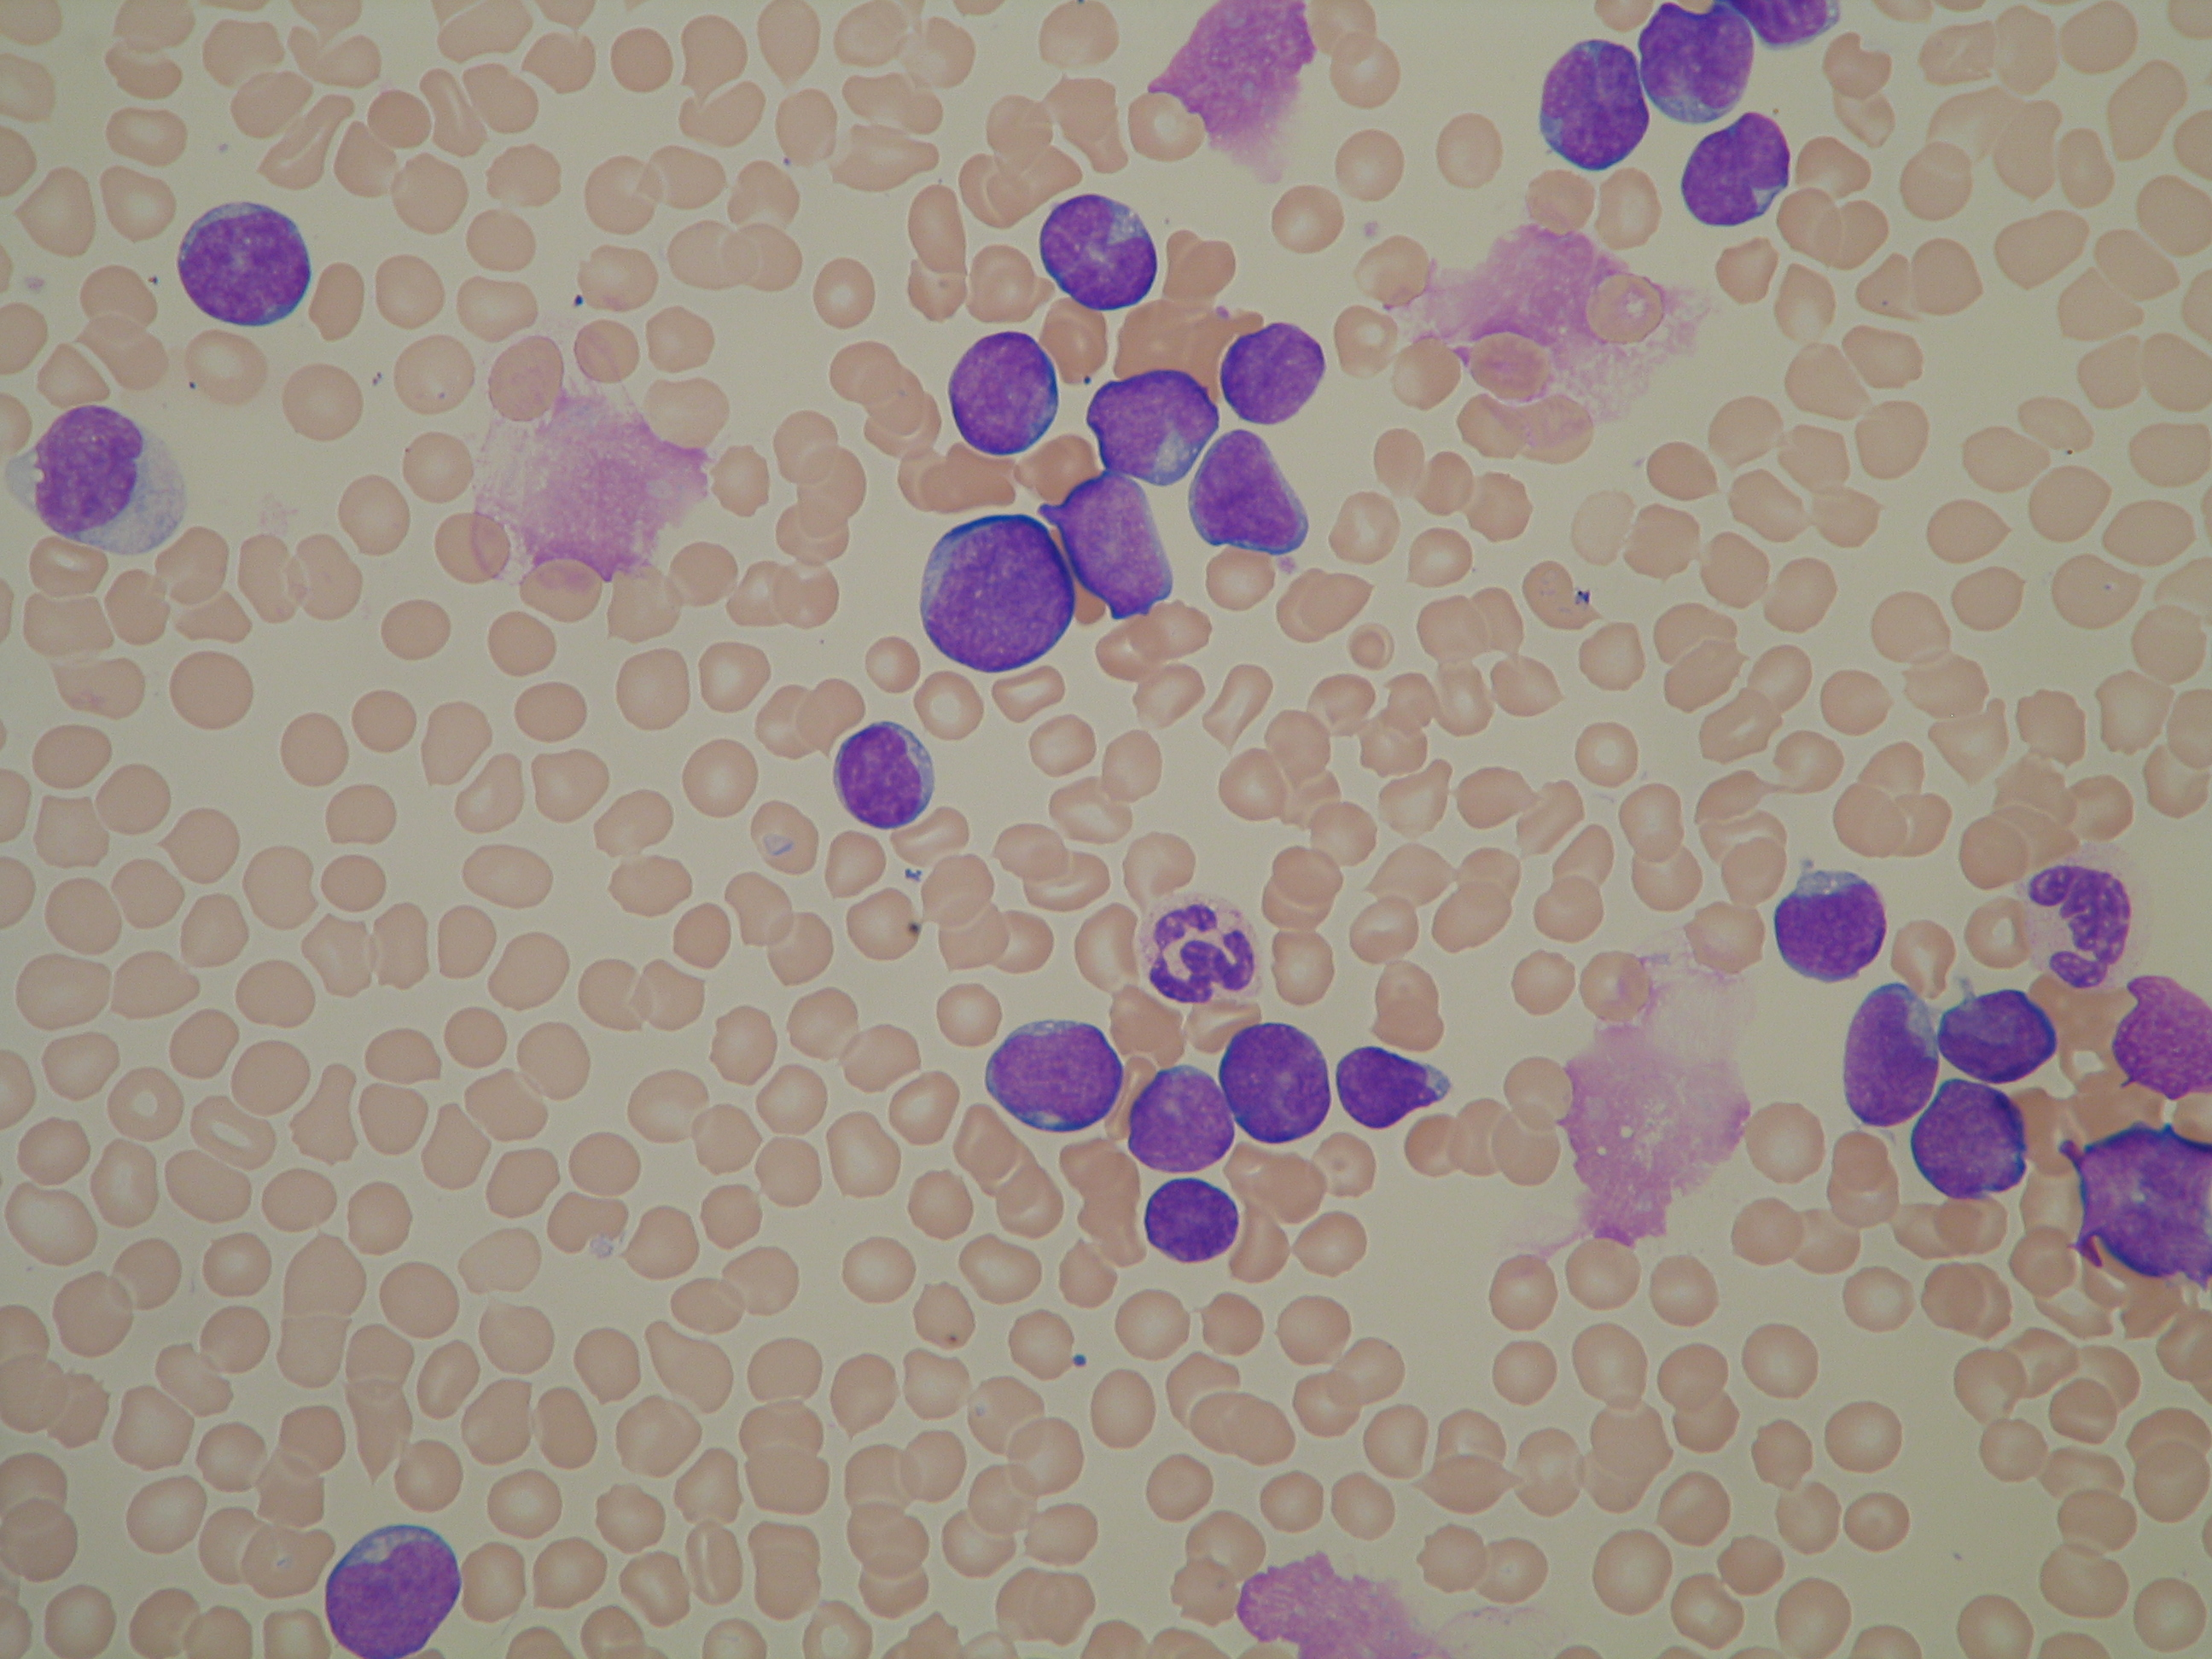
\includegraphics[width=3cm]{images/Im058_1.jpg}}
  \quad  
  \subfloat[]{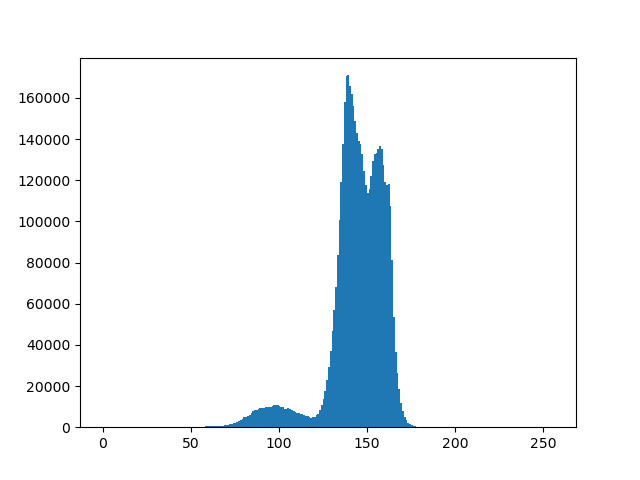
\includegraphics[width=3cm]{images/Im048_hist.png}}
  \quad 
  \subfloat[]{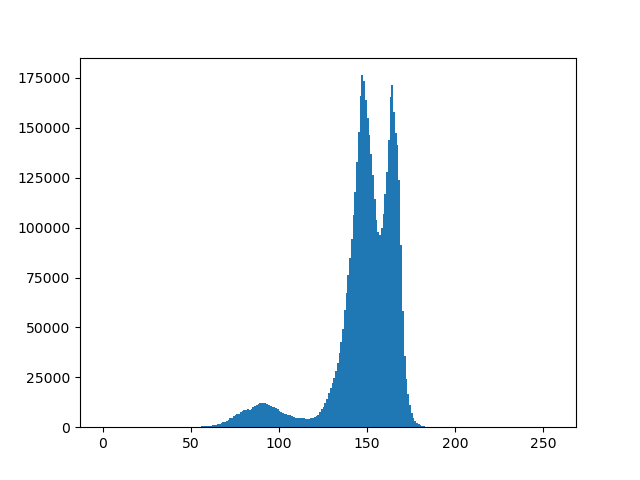
\includegraphics[width=3cm]{images/Im058_hist.png}}
  \quad  
  \caption{(c) and (d) are pixel color frequency histograms of the blood microscopic images (a) and (b)}
\end{figure}

\subsection{Process}

The proposed pipeline is composed of four steps. We start by thresholding input images to generate a mask that will be used to extract white blood cells from blood microscopic images. The regions of interest are, then, fed into pre-trained CNNs, and our proposed lightweight network. As state-of-the-art networks, we select ResNet50 \cite{he2016deep} and RegNet \cite{radosavovic2020designing} which are pre-trained using the ImageNet 1k dataset. The proposed lightweight CNN architecture is composed of two convolutional layers each one is preceded by a max pooling layer with 2 kernel size and 2 stride value in order to reduce the computations. The FCN is made of dense, ELU, dropout, and Softmax layers. We use the ELU to deal with the vanishing gradient problem, a 0.2 dropout rate for overfitting, and two output neurons within the output layer. 
We train our networks using the cross entropy loss function, an Adam optimizer, and 1e-4 learning rate. 
To test our models using the whole dataset, we use the four-fold cross-validation technique. The accuracy, the precision, the recall, and the f1-score are used as metrics to evaluate the performance of different methods.
\begin{figure}[!h]
  \centering
  \subfloat[]{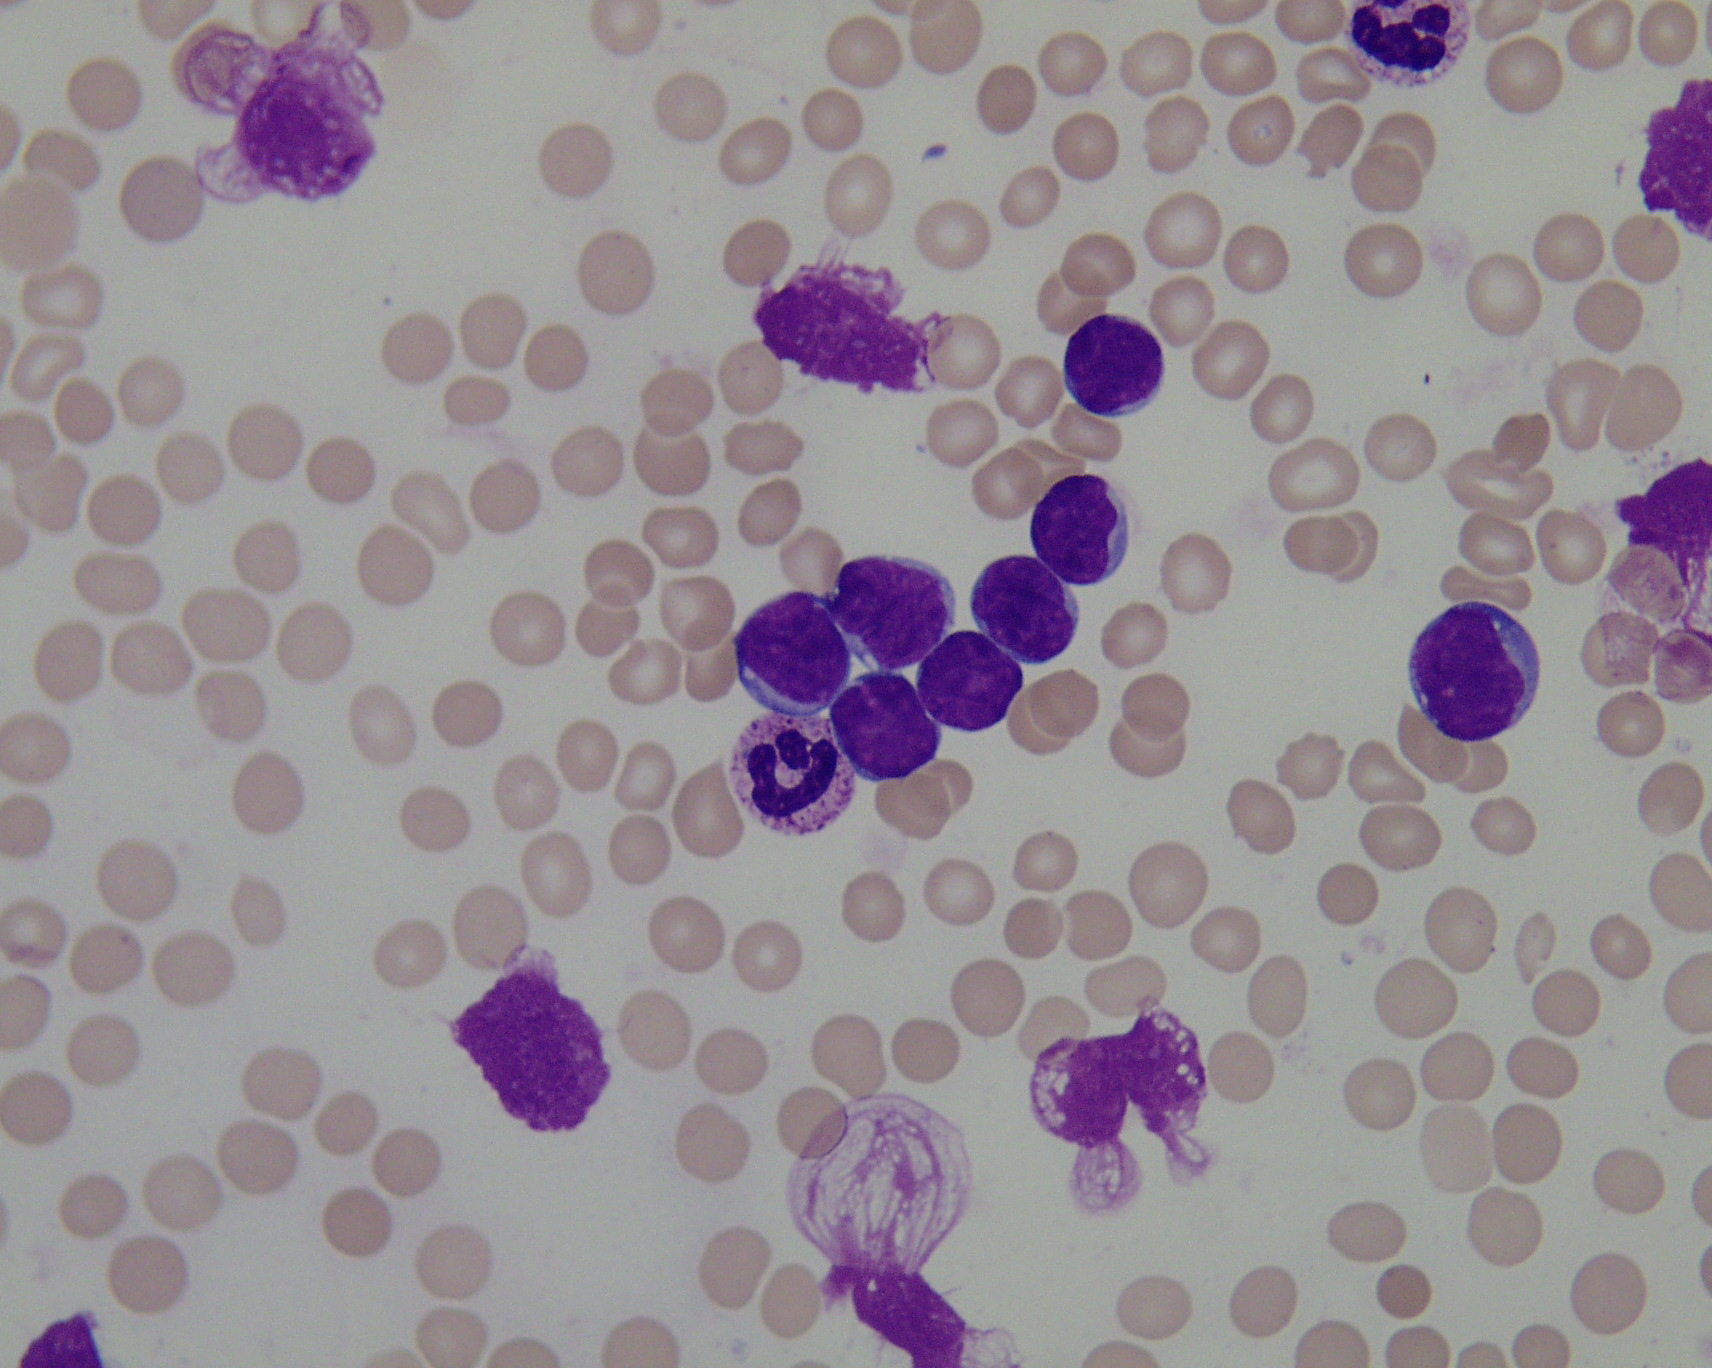
\includegraphics[width=3cm]{images/Im001_1.jpg}}
  \quad 
  \subfloat[]{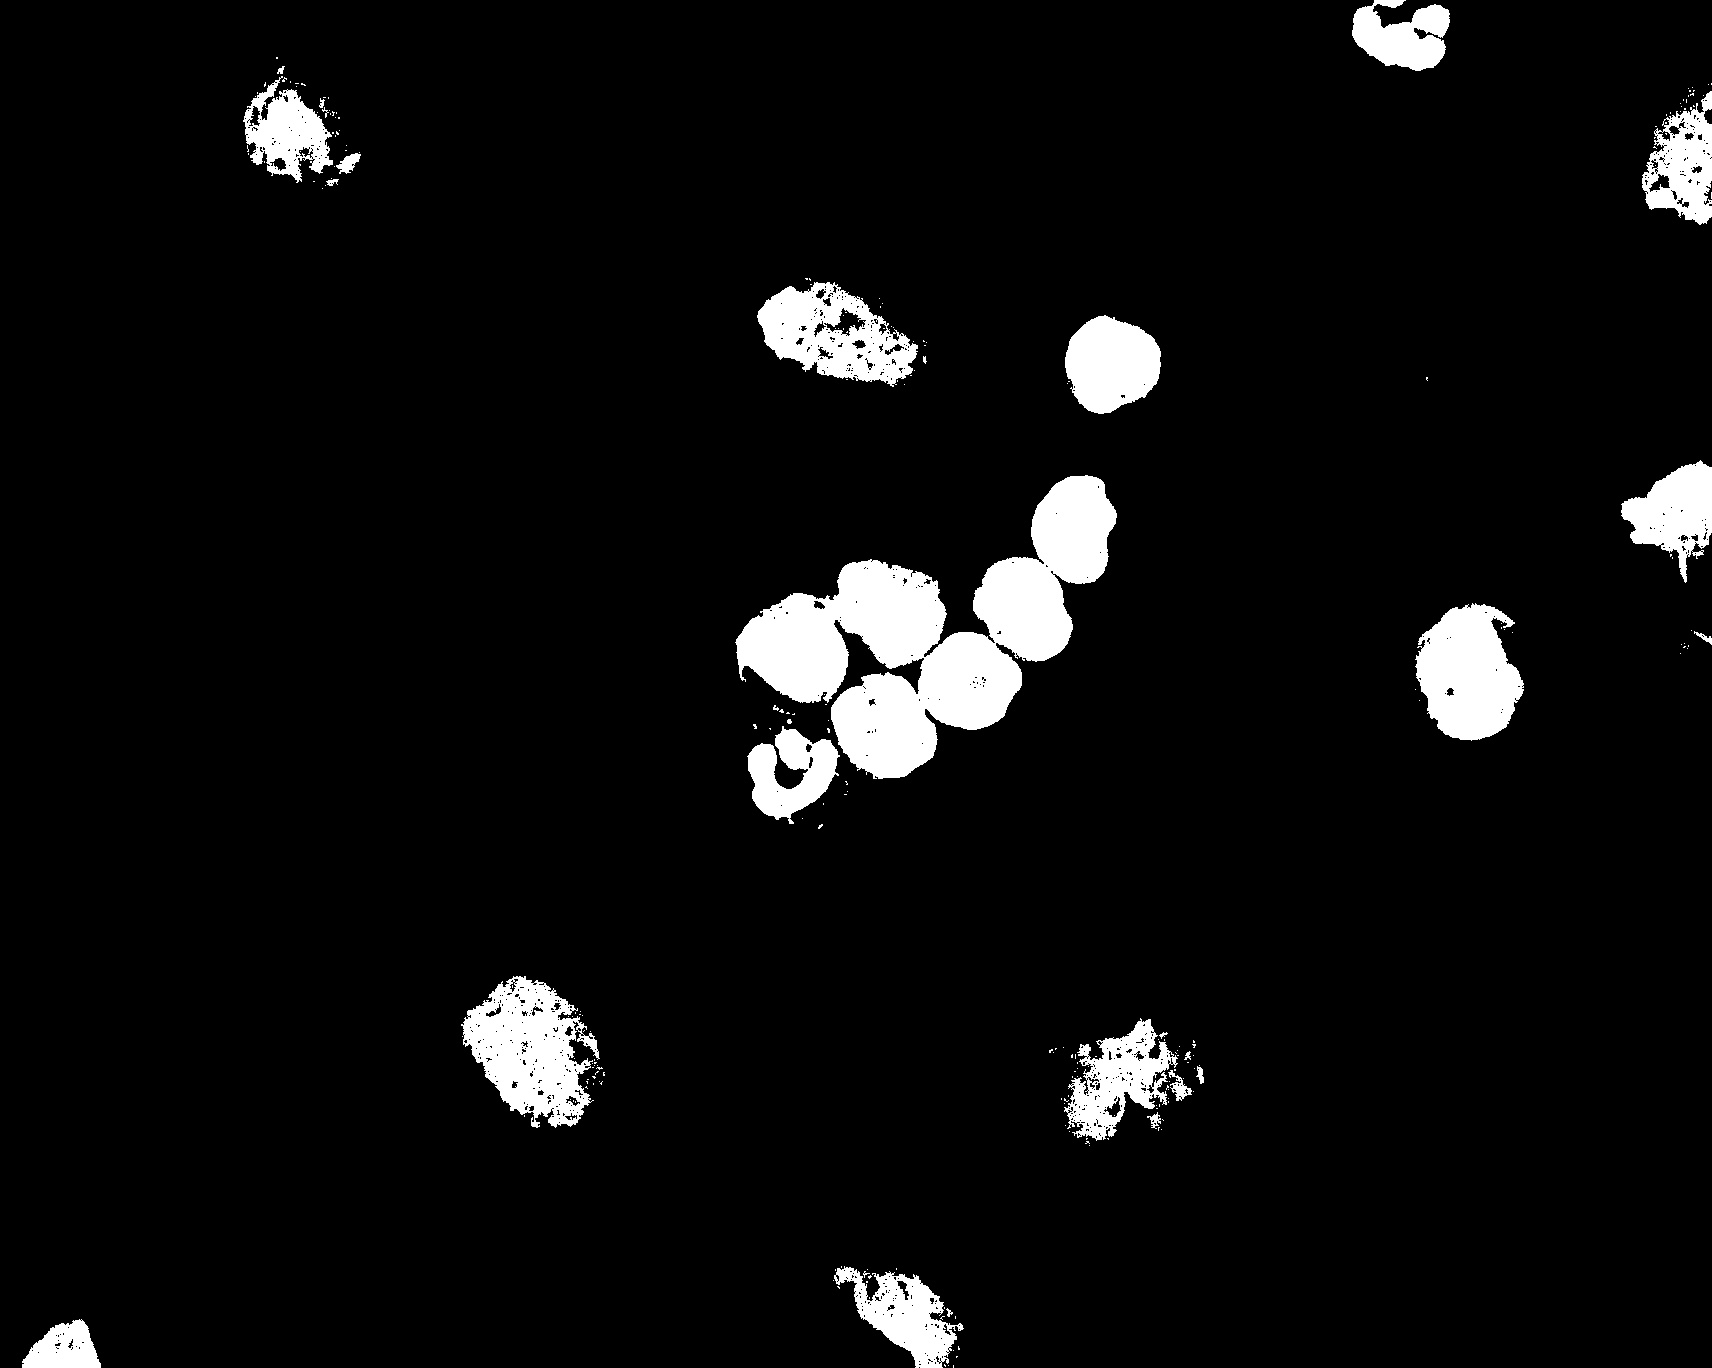
\includegraphics[width=3cm]{images/Im001_1 (1).jpg}}
  \quad 
  \subfloat[]{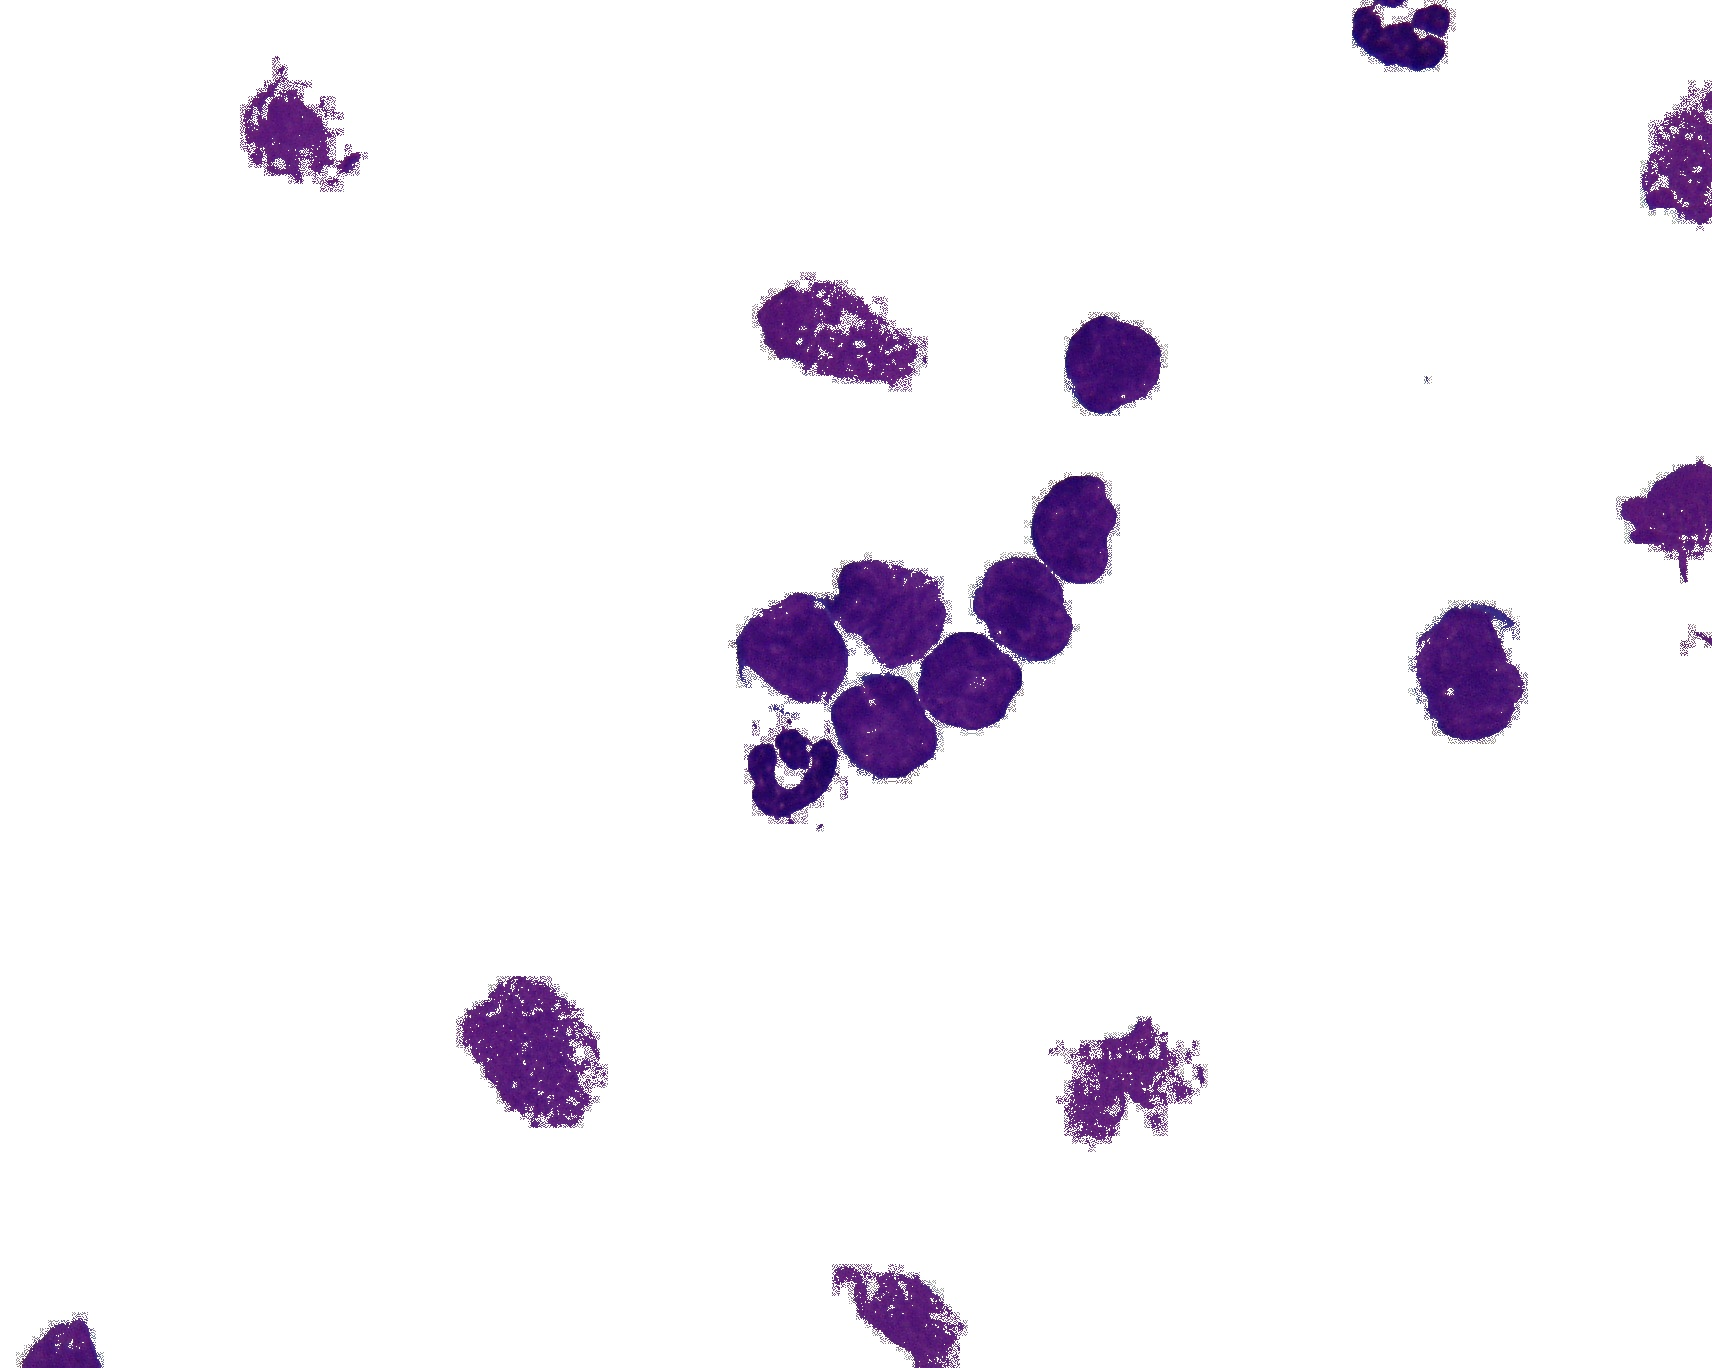
\includegraphics[width=3cm]{images/Im001_1 (2).jpg}}
  \quad  
  \caption{(a) is a blood microscopic image containing leukocytes. (b) is the mask of (a) generated using binary thresholding. (c) are the extracted lymphocytes using mask (b)}
\end{figure}

\section{Results and Findings}
Our models are trained using an Intel® Core™ i7-10870H CPU and NVIDIA Corporation GA107M GPU. We used the Pytorch library to implement the deep learning algorithm.

Table 1 shows the performance of the deep learning models recorded on the ALL-IDB1 and ALL-IDB2 datasets. The proposed CNN outperformed all other models while scoring an accuracy of 99\%, a precision of 99\%, a recall of 99\%, and an F1-score of 99\%.  On the other hand, the pre-trained ResNet50 model registered an accuracy of 96\%, a precision of 96\%, a recall of 96\%, and an F1-score of 96\%. The proposed lightweight CNN outperformed other models because it has a less deep architecture and few convolutional layers that can fit a small dataset.

\begin{table}[h!]
  \centering
  \caption{The recorded performance of deep learning models on the ALL-IDB1 and ALL-IDB2 datasets}
  \begin{adjustbox}{width=\columnwidth,center}
    \begin{tabular}{c c c  c  c  c c}
      \hline
      Model & dataset & epochs & Accuracy(\%) & Precision(\%) & Recall(\%) & F1-score (\%)\\ [0.5ex]
      \hline
      ResNet50 & ALL-IDB 1 & 25 & 96 & 96 & 96 & 96\\
      RegNet & ALL-IDB 1 & 25 & 97 & 97 & 97 & 97 \\
      Proposed CNN & ALL-IDB 1 & 25 & 99 & 99 & 99 & 99 \\
      ResNet50 & ALL-IDB 2 & 25 & 98 & 98 & 98 & 98\\
      RegNet & ALL-IDB 2 & 25 & 98 & 98 & 98 & 98 \\
      Proposed CNN & ALL-IDB 2 & 25 & 98 & 98 & 98 & 98 \\
      \hline
    \end{tabular}
  \end{adjustbox}
  \label{table:1}
\end{table}



Figure 4 shows the confusion matrices (CM) of the proposed lightwright CNN and the ResNet model recorded on the ALL-IDB 1 and ALL-IDB 2 dataset. For instance, in the first CM, all samples belonging to the leukemia class are correctly classified. The false negative value is 1 meaning that only one patient is misclassified as having leukemia while he is healthy.  The true negative value is 48.

\begin{figure}[!h]
  \centering
  \subfloat[]{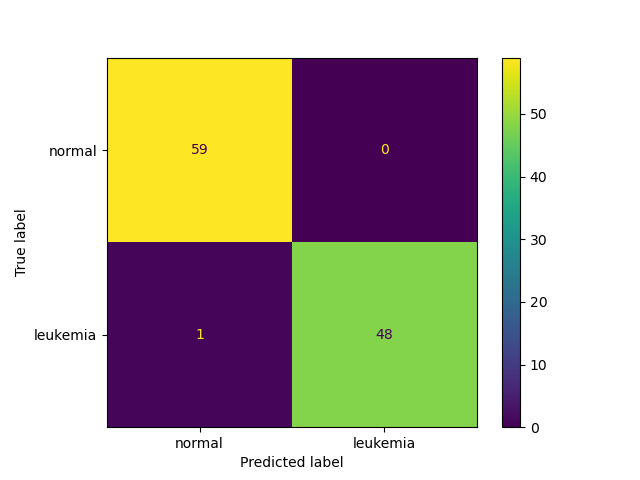
\includegraphics[width=4.5cm]{images/LightCNN_CM.png}}
  \quad 
  \subfloat[]{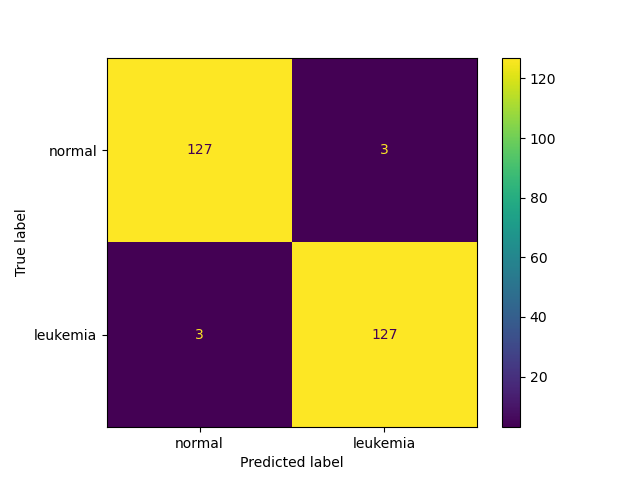
\includegraphics[width=4.5cm]{images/LightCNN_CM_allidb2.png}}
  \quad  
  \subfloat[]{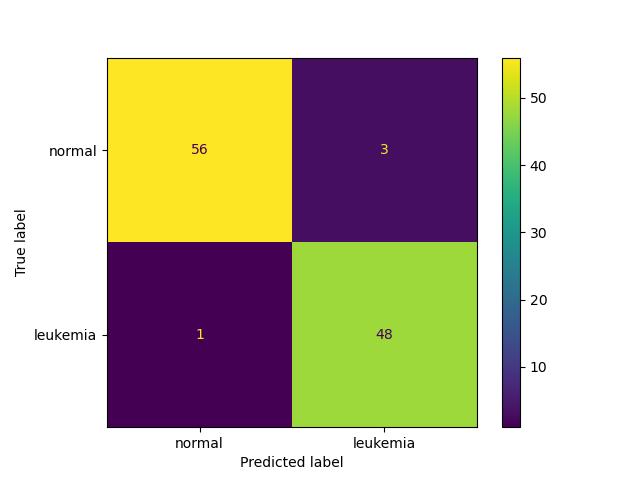
\includegraphics[width=4.5cm]{images/Resnet_CM.png}}
  \quad 
  \subfloat[]{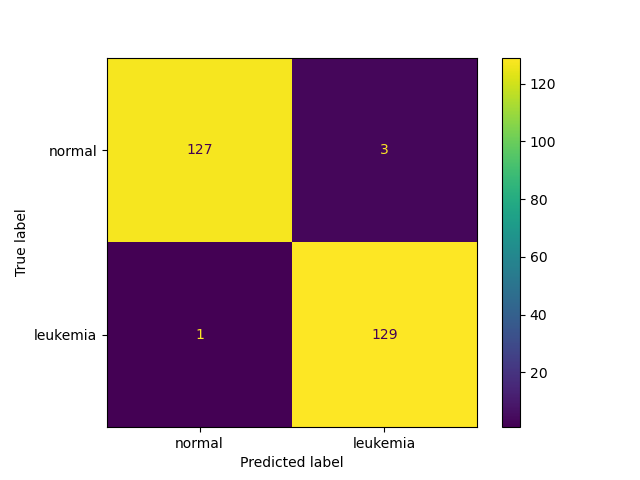
\includegraphics[width=4.5cm]{images/ResNet_CM_allidb2.png}}
  \quad  
  \caption{ The confuxion matrices of the proposed models. (a) and (b) are the CM for the proposed model on both datasets and (c) and (d) are the CM of the ResNet model respectively on the ALL-IDB 1 and ALL-IDB 2. }
\end{figure}

\newpage

Figure 5 shows the misclassified sample in the confusion matrix (a). We notice that there are few lymphocyte cells and this is the reason why the model considers the sample as normal while it is from a patient suffering from leukemia.

\begin{figure}[!h]
  \centering
 
  \subfloat[]{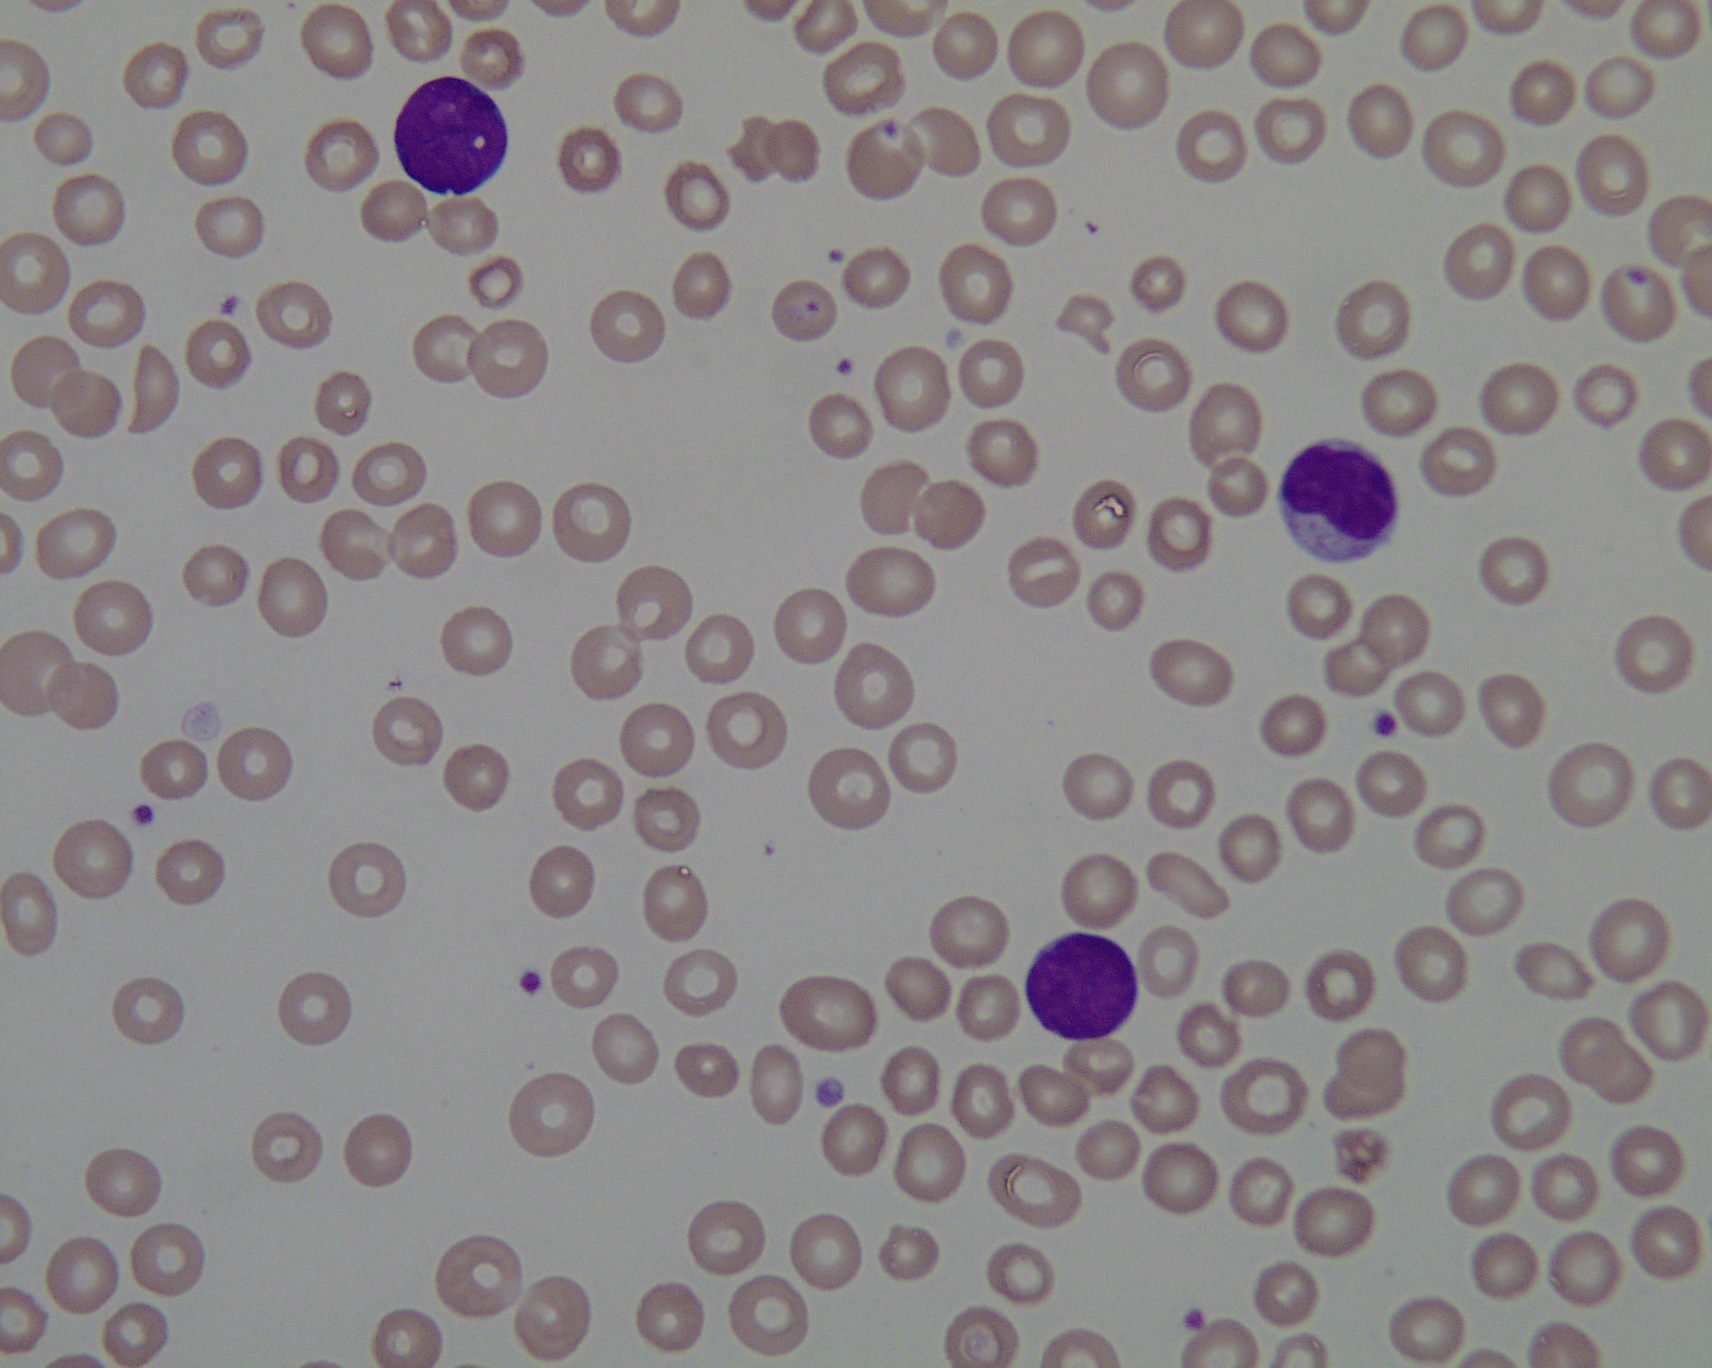
\includegraphics[width=3cm]{images/Im025_1.jpg}}
  \quad 
  \subfloat[]{
\includegraphics[width=3cm]{images/Im025_1 (1).jpg}}
  \quad  
  \caption{(a) is the microscopic images that is misclassified by the proposed model and (b) is the region of interest fed into the network}
\end{figure}

\section{Conclusion}
This study introduced a CADx system to detect leukemia from blood microscopic images. The proposed method outperformed all models within the literature. The best performance is recorded on the ALL-IDB 1 dataset where the model manages to classify all the samples correctly except for one image. We further investigate the reason why the model is misclassifying this sample and we found that there are few lymphocytes in the microscopic image. This means that the proposed algorithm is imlicitly taking into consideration the number of white blood cells within the image. The novelty of our work consists of the thresholding method and the lightweight CNN architecture.

In further studies, we propose the use of object detection networks that try to predict the coordinates of lymphocytes and classify them as either normal or leukocytes.

\begin{adjustwidth}{-\extralength}{0cm}
	%\printendnotes[custom] % Un-comment to print a list of endnotes
	
\reftitle{References}
\bibliography{refs}

% If authors have biography, please use the format below
%\section*{Short Biography of Authors}
%\bio
%{\raisebox{-0.35cm}{\includegraphics[width=3.5cm,height=5.3cm,clip,keepaspectratio]{Definitions/author1.pdf}}}
%{\textbf{Firstname Lastname} Biography of first author}
%
%\bio
%{\raisebox{-0.35cm}{\includegraphics[width=3.5cm,height=5.3cm,clip,keepaspectratio]{Definitions/author2.jpg}}}
%{\textbf{Firstname Lastname} Biography of second author}

% For the MDPI journals use author-date citation, please follow the formatting guidelines on http://www.mdpi.com/authors/references
% To cite two works by the same author: \citeauthor{ref-journal-1a} (\citeyear{ref-journal-1a}, \citeyear{ref-journal-1b}). This produces: Whittaker (1967, 1975)
% To cite two works by the same author with specific pages: \citeauthor{ref-journal-3a} (\citeyear{ref-journal-3a}, p. 328; \citeyear{ref-journal-3b}, p.475). This produces: Wong (1999, p. 328; 2000, p. 475)

%%%%%%%%%%%%%%%%%%%%%%%%%%%%%%%%%%%%%%%%%%
%% for journal Sci
%\reviewreports{\\
%Reviewer 1 comments and authors’ response\\
%Reviewer 2 comments and authors’ response\\
%Reviewer 3 comments and authors’ response
%}
%%%%%%%%%%%%%%%%%%%%%%%%%%%%%%%%%%%%%%%%%%
\PublishersNote{}
\end{adjustwidth}
\end{document}

